\documentclass[1p]{elsarticle_modified}
%\bibliographystyle{elsarticle-num}

%\usepackage[colorlinks]{hyperref}
%\usepackage{abbrmath_seonhwa} %\Abb, \Ascr, \Acal ,\Abf, \Afrak
\usepackage{amsfonts}
\usepackage{amssymb}
\usepackage{amsmath}
\usepackage{amsthm}
\usepackage{scalefnt}
\usepackage{amsbsy}
\usepackage{kotex}
\usepackage{caption}
\usepackage{subfig}
\usepackage{color}
\usepackage{graphicx}
\usepackage{xcolor} %% white, black, red, green, blue, cyan, magenta, yellow
\usepackage{float}
\usepackage{setspace}
\usepackage{hyperref}

\usepackage{tikz}
\usetikzlibrary{arrows}

\usepackage{multirow}
\usepackage{array} % fixed length table
\usepackage{hhline}

%%%%%%%%%%%%%%%%%%%%%
\makeatletter
\renewcommand*\env@matrix[1][\arraystretch]{%
	\edef\arraystretch{#1}%
	\hskip -\arraycolsep
	\let\@ifnextchar\new@ifnextchar
	\array{*\c@MaxMatrixCols c}}
\makeatother %https://tex.stackexchange.com/questions/14071/how-can-i-increase-the-line-spacing-in-a-matrix
%%%%%%%%%%%%%%%

\usepackage[normalem]{ulem}

\newcommand{\msout}[1]{\ifmmode\text{\sout{\ensuremath{#1}}}\else\sout{#1}\fi}
%SOURCE: \msout is \stkout macro in https://tex.stackexchange.com/questions/20609/strikeout-in-math-mode

\newcommand{\cancel}[1]{
	\ifmmode
	{\color{red}\msout{#1}}
	\else
	{\color{red}\sout{#1}}
	\fi
}

\newcommand{\add}[1]{
	{\color{blue}\uwave{#1}}
}

\newcommand{\replace}[2]{
	\ifmmode
	{\color{red}\msout{#1}}{\color{blue}\uwave{#2}}
	\else
	{\color{red}\sout{#1}}{\color{blue}\uwave{#2}}
	\fi
}

\newcommand{\Sol}{\mathcal{S}} %segment
\newcommand{\D}{D} %diagram
\newcommand{\A}{\mathcal{A}} %arc


%%%%%%%%%%%%%%%%%%%%%%%%%%%%%5 test

\def\sl{\operatorname{\textup{SL}}(2,\Cbb)}
\def\psl{\operatorname{\textup{PSL}}(2,\Cbb)}
\def\quan{\mkern 1mu \triangleright \mkern 1mu}

\theoremstyle{definition}
\newtheorem{thm}{Theorem}[section]
\newtheorem{prop}[thm]{Proposition}
\newtheorem{lem}[thm]{Lemma}
\newtheorem{ques}[thm]{Question}
\newtheorem{cor}[thm]{Corollary}
\newtheorem{defn}[thm]{Definition}
\newtheorem{exam}[thm]{Example}
\newtheorem{rmk}[thm]{Remark}
\newtheorem{alg}[thm]{Algorithm}

\newcommand{\I}{\sqrt{-1}}
\begin{document}

%\begin{frontmatter}
%
%\title{Boundary parabolic representations of knots up to 8 crossings}
%
%%% Group authors per affiliation:
%\author{Yunhi Cho} 
%\address{Department of Mathematics, University of Seoul, Seoul, Korea}
%\ead{yhcho@uos.ac.kr}
%
%
%\author{Seonhwa Kim} %\fnref{s_kim}}
%\address{Center for Geometry and Physics, Institute for Basic Science, Pohang, 37673, Korea}
%\ead{ryeona17@ibs.re.kr}
%
%\author{Hyuk Kim}
%\address{Department of Mathematical Sciences, Seoul National University, Seoul 08826, Korea}
%\ead{hyukkim@snu.ac.kr}
%
%\author{Seokbeom Yoon}
%\address{Department of Mathematical Sciences, Seoul National University, Seoul, 08826,  Korea}
%\ead{sbyoon15@snu.ac.kr}
%
%\begin{abstract}
%We find all boundary parabolic representation of knots up to 8 crossings.
%
%\end{abstract}
%\begin{keyword}
%    \MSC[2010] 57M25 
%\end{keyword}
%
%\end{frontmatter}

%\linenumbers
%\tableofcontents
%
\newcommand\colored[1]{\textcolor{white}{\rule[-0.35ex]{0.8em}{1.4ex}}\kern-0.8em\color{red} #1}%
%\newcommand\colored[1]{\textcolor{white}{ #1}\kern-2.17ex	\textcolor{white}{ #1}\kern-1.81ex	\textcolor{white}{ #1}\kern-2.15ex\color{red}#1	}

{\Large $\underline{11a_{160}~(K11a_{160})}$}

\setlength{\tabcolsep}{10pt}
\renewcommand{\arraystretch}{1.6}
\vspace{1cm}\begin{tabular}{m{100pt}>{\centering\arraybackslash}m{274pt}}
\multirow{5}{120pt}{
	\centering
	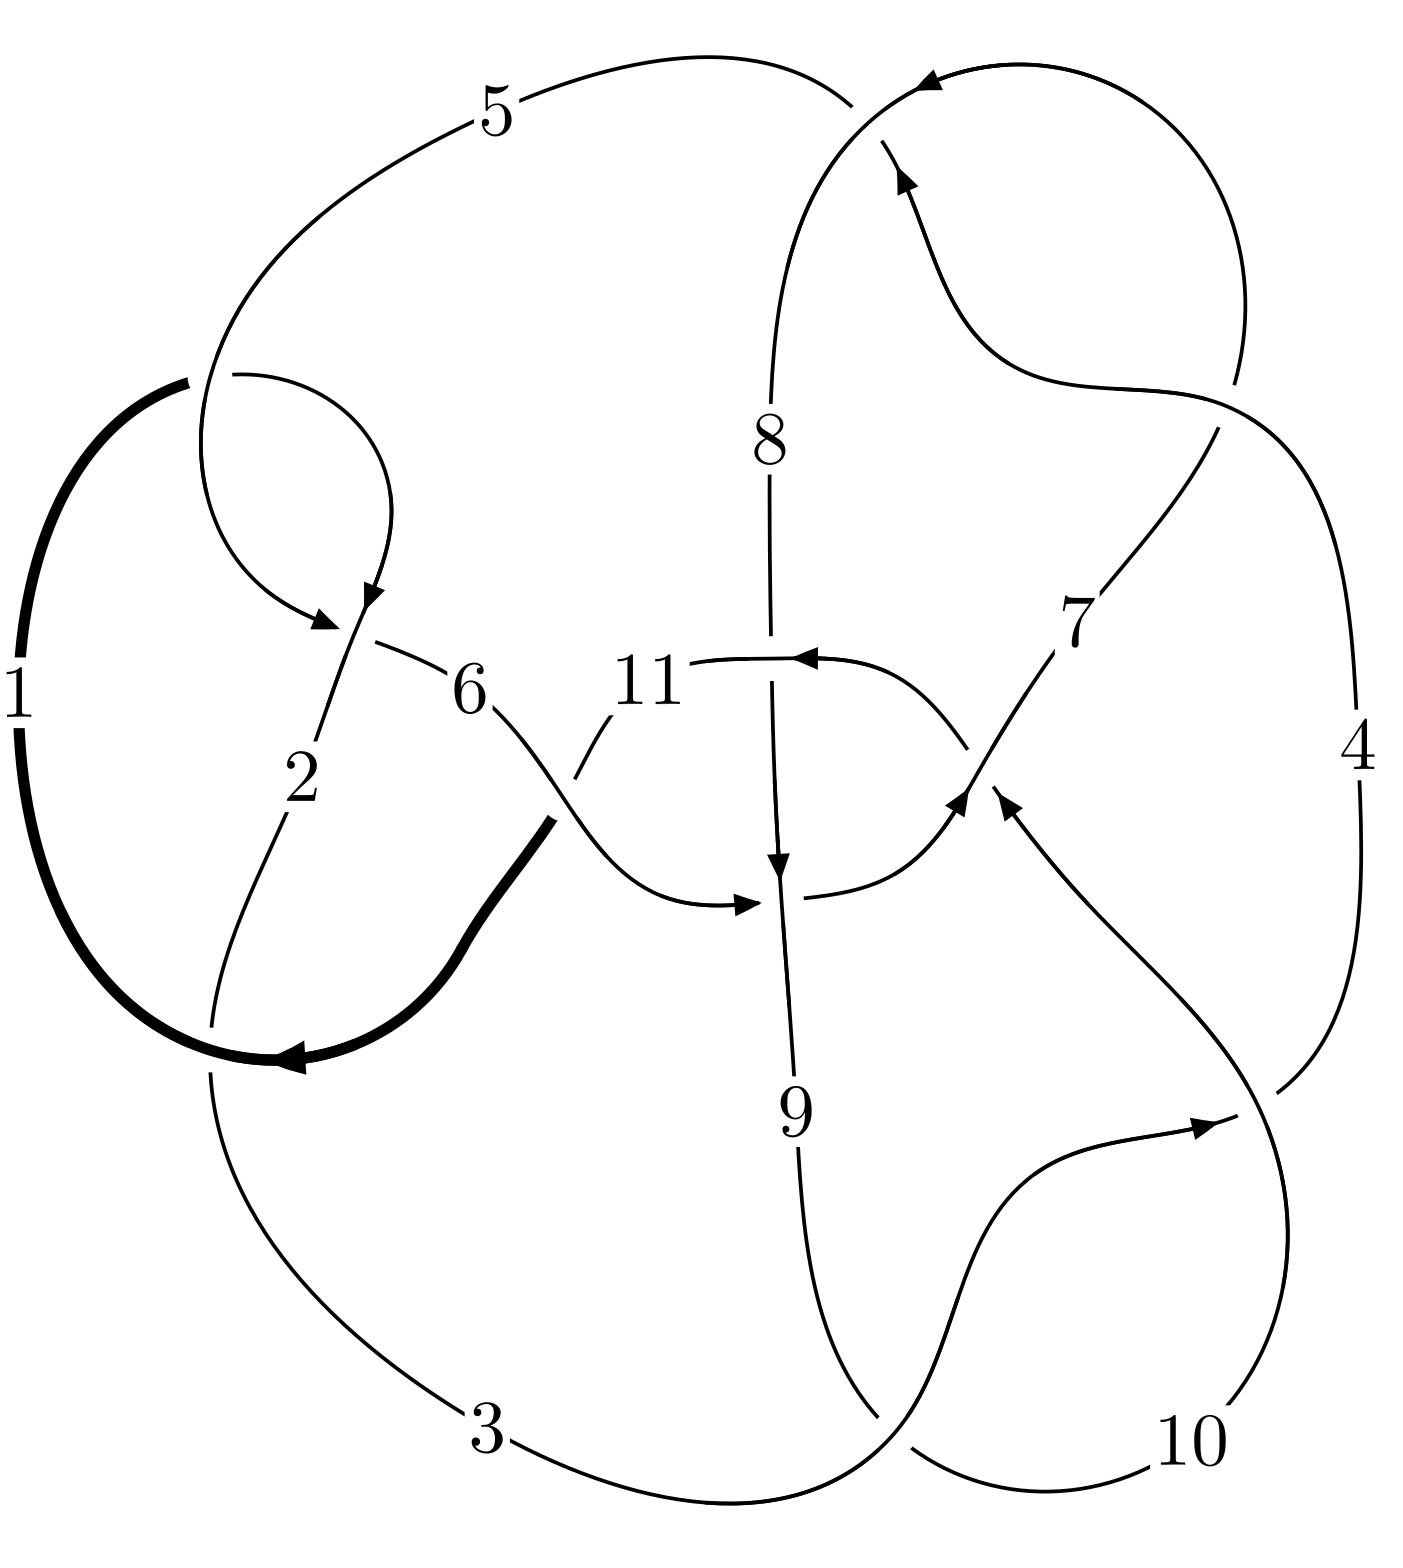
\includegraphics[width=112pt]{../../../GIT/diagram.site/Diagrams/png/409_11a_160.png}\\
\ \ \ A knot diagram\footnotemark}&
\allowdisplaybreaks
\textbf{Linearized knot diagam} \\
\cline{2-2}
 &
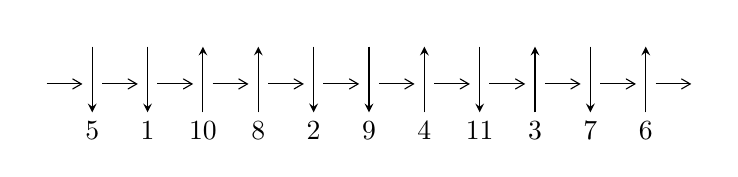
\begin{tikzpicture}[x=20pt, y=17pt]
	% nodes
	\node (C0) at (0, 0) {};
	\node (C1) at (1, 0) {};
	\node (C1U) at (1, +1) {};
	\node (C1D) at (1, -1) {5};

	\node (C2) at (2, 0) {};
	\node (C2U) at (2, +1) {};
	\node (C2D) at (2, -1) {1};

	\node (C3) at (3, 0) {};
	\node (C3U) at (3, +1) {};
	\node (C3D) at (3, -1) {10};

	\node (C4) at (4, 0) {};
	\node (C4U) at (4, +1) {};
	\node (C4D) at (4, -1) {8};

	\node (C5) at (5, 0) {};
	\node (C5U) at (5, +1) {};
	\node (C5D) at (5, -1) {2};

	\node (C6) at (6, 0) {};
	\node (C6U) at (6, +1) {};
	\node (C6D) at (6, -1) {9};

	\node (C7) at (7, 0) {};
	\node (C7U) at (7, +1) {};
	\node (C7D) at (7, -1) {4};

	\node (C8) at (8, 0) {};
	\node (C8U) at (8, +1) {};
	\node (C8D) at (8, -1) {11};

	\node (C9) at (9, 0) {};
	\node (C9U) at (9, +1) {};
	\node (C9D) at (9, -1) {3};

	\node (C10) at (10, 0) {};
	\node (C10U) at (10, +1) {};
	\node (C10D) at (10, -1) {7};

	\node (C11) at (11, 0) {};
	\node (C11U) at (11, +1) {};
	\node (C11D) at (11, -1) {6};
	\node (C12) at (12, 0) {};

	% arrows
	\draw[->,>={angle 60}]
	(C0) edge (C1) (C1) edge (C2) (C2) edge (C3) (C3) edge (C4) (C4) edge (C5) (C5) edge (C6) (C6) edge (C7) (C7) edge (C8) (C8) edge (C9) (C9) edge (C10) (C10) edge (C11) (C11) edge (C12) ;	\draw[->,>=stealth]
	(C1U) edge (C1D) (C2U) edge (C2D) (C3D) edge (C3U) (C4D) edge (C4U) (C5U) edge (C5D) (C6U) edge (C6D) (C7D) edge (C7U) (C8U) edge (C8D) (C9D) edge (C9U) (C10U) edge (C10D) (C11D) edge (C11U) ;
	\end{tikzpicture} \\
\hhline{~~} \\& 
\textbf{Solving Sequence} \\ \cline{2-2} 
 &
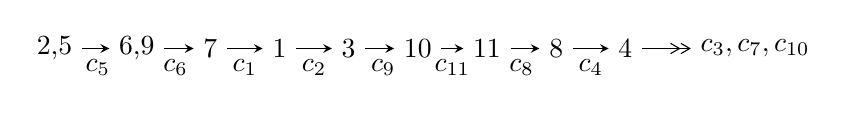
\begin{tikzpicture}[x=25pt, y=7pt]
	% node
	\node (A0) at (-1/8, 0) {2,5};
	\node (A1) at (17/16, 0) {6,9};
	\node (A2) at (17/8, 0) {7};
	\node (A3) at (25/8, 0) {1};
	\node (A4) at (33/8, 0) {3};
	\node (A5) at (41/8, 0) {10};
	\node (A6) at (49/8, 0) {11};
	\node (A7) at (57/8, 0) {8};
	\node (A8) at (65/8, 0) {4};
	\node (C1) at (1/2, -1) {$c_{5}$};
	\node (C2) at (13/8, -1) {$c_{6}$};
	\node (C3) at (21/8, -1) {$c_{1}$};
	\node (C4) at (29/8, -1) {$c_{2}$};
	\node (C5) at (37/8, -1) {$c_{9}$};
	\node (C6) at (45/8, -1) {$c_{11}$};
	\node (C7) at (53/8, -1) {$c_{8}$};
	\node (C8) at (61/8, -1) {$c_{4}$};
	\node (A9) at (10, 0) {$c_{3},c_{7},c_{10}$};

	% edge
	\draw[->,>=stealth]	
	(A0) edge (A1) (A1) edge (A2) (A2) edge (A3) (A3) edge (A4) (A4) edge (A5) (A5) edge (A6) (A6) edge (A7) (A7) edge (A8) ;
	\draw[->>,>={angle 60}]	
	(A8) edge (A9);
\end{tikzpicture} \\ 

\end{tabular} \\

\footnotetext{
The image of knot diagram is generated by the software ``\textbf{Draw programme}" developed by Andrew Bartholomew(\url{http://www.layer8.co.uk/maths/draw/index.htm\#Running-draw}), where we modified some parts for our purpose(\url{https://github.com/CATsTAILs/LinksPainter}).
}\phantom \\ \newline 
\centering \textbf{Ideals for irreducible components\footnotemark of $X_{\text{par}}$} 
 
\begin{align*}
I^u_{1}&=\langle 
-5 u^{29}-20 u^{28}+\cdots+2 b-14,\;3 u^{29}+16 u^{28}+\cdots+4 a-9 u,\;u^{30}+6 u^{29}+\cdots+26 u+4\rangle \\
I^u_{2}&=\langle 
4584333581 u^{13} a^3+6949760010 u^{13} a^2+\cdots-45118851 a-4067169136,\\
\phantom{I^u_{2}}&\phantom{= \langle  }-2 u^{13} a^3-2 u^{13} a^2+\cdots+a-4,\;u^{14}- u^{13}-3 u^{12}+4 u^{11}+4 u^{10}-7 u^9- u^8+6 u^7-2 u^6-2 u^5+2 u^4- u+1\rangle \\
I^u_{3}&=\langle 
u^{12}+u^{11}-3 u^{10}-2 u^9+5 u^8+2 u^7-3 u^6+u^5+2 u^4-2 u^3-2 u^2+b+u+2,\\
\phantom{I^u_{3}}&\phantom{= \langle  }- u^{13}+u^{12}+5 u^{11}-4 u^{10}-9 u^9+8 u^8+8 u^7-9 u^6+9 u^4-4 u^3-6 u^2+a+2 u+3,\\
\phantom{I^u_{3}}&\phantom{= \langle  }u^{14}- u^{13}-3 u^{12}+4 u^{11}+4 u^{10}-7 u^9- u^8+7 u^7-3 u^6-4 u^5+4 u^4+2 u^3-2 u^2- u+1\rangle \\
\\
\end{align*}
\raggedright * 3 irreducible components of $\dim_{\mathbb{C}}=0$, with total 100 representations.\\
\footnotetext{All coefficients of polynomials are rational numbers. But the coefficients are sometimes approximated in decimal forms when there is not enough margin.}
\newpage
\renewcommand{\arraystretch}{1}
\centering \section*{I. $I^u_{1}= \langle -5 u^{29}-20 u^{28}+\cdots+2 b-14,\;3 u^{29}+16 u^{28}+\cdots+4 a-9 u,\;u^{30}+6 u^{29}+\cdots+26 u+4 \rangle$}
\flushleft \textbf{(i) Arc colorings}\\
\begin{tabular}{m{7pt} m{180pt} m{7pt} m{180pt} }
\flushright $a_{2}=$&$\begin{pmatrix}0\\u\end{pmatrix}$ \\
\flushright $a_{5}=$&$\begin{pmatrix}1\\0\end{pmatrix}$ \\
\flushright $a_{6}=$&$\begin{pmatrix}1\\u^2\end{pmatrix}$ \\
\flushright $a_{9}=$&$\begin{pmatrix}-\frac{3}{4} u^{29}-4 u^{28}+\cdots-2 u^2+\frac{9}{4} u\\\frac{5}{2} u^{29}+10 u^{28}+\cdots+\frac{77}{2} u+7\end{pmatrix}$ \\
\flushright $a_{7}=$&$\begin{pmatrix}-7 u^{29}-\frac{69}{2} u^{28}+\cdots-133 u-\frac{43}{2}\\-\frac{11}{2} u^{29}-29 u^{28}+\cdots-\frac{289}{2} u-26\end{pmatrix}$ \\
\flushright $a_{1}=$&$\begin{pmatrix}u\\u\end{pmatrix}$ \\
\flushright $a_{3}=$&$\begin{pmatrix}- u^3\\- u^3+u\end{pmatrix}$ \\
\flushright $a_{10}=$&$\begin{pmatrix}\frac{17}{4} u^{29}+26 u^{28}+\cdots+\frac{625}{4} u+28\\\frac{1}{2} u^{29}+5 u^{28}+\cdots+\frac{97}{2} u+9\end{pmatrix}$ \\
\flushright $a_{11}=$&$\begin{pmatrix}u^3\\u^5- u^3+u\end{pmatrix}$ \\
\flushright $a_{8}=$&$\begin{pmatrix}\frac{29}{4} u^{29}+34 u^{28}+\cdots+\frac{497}{4} u+20\\\frac{13}{2} u^{29}+32 u^{28}+\cdots+\frac{281}{2} u+25\end{pmatrix}$ \\
\flushright $a_{4}=$&$\begin{pmatrix}u^{29}+\frac{3}{2} u^{28}+\cdots-29 u-\frac{11}{2}\\\frac{11}{2} u^{29}+27 u^{28}+\cdots+\frac{157}{2} u+12\end{pmatrix}$\\ \flushright $a_{4}=$&$\begin{pmatrix}u^{29}+\frac{3}{2} u^{28}+\cdots-29 u-\frac{11}{2}\\\frac{11}{2} u^{29}+27 u^{28}+\cdots+\frac{157}{2} u+12\end{pmatrix}$\\&\end{tabular}
\flushleft \textbf{(ii) Obstruction class $= -1$}\\~\\
\flushleft \textbf{(iii) Cusp Shapes $= 2 u^{29}+12 u^{28}+8 u^{27}-69 u^{26}-140 u^{25}+91 u^{24}+537 u^{23}+337 u^{22}-834 u^{21}-1449 u^{20}-13 u^{19}+2090 u^{18}+1957 u^{17}-581 u^{16}-2559 u^{15}-1877 u^{14}+350 u^{13}+1886 u^{12}+1755 u^{11}+441 u^{10}-966 u^9-1388 u^8-688 u^7+298 u^6+655 u^5+378 u^4-5 u^3-123 u^2-80 u-22$}\\~\\
\newpage\renewcommand{\arraystretch}{1}
\flushleft \textbf{(iv) u-Polynomials at the component}\newline \\
\begin{tabular}{m{50pt}|m{274pt}}
Crossings & \hspace{64pt}u-Polynomials at each crossing \\
\hline $$\begin{aligned}c_{1},c_{5}\end{aligned}$$&$\begin{aligned}
&u^{30}+6 u^{29}+\cdots+26 u+4
\end{aligned}$\\
\hline $$\begin{aligned}c_{2}\end{aligned}$$&$\begin{aligned}
&u^{30}+14 u^{29}+\cdots+28 u+16
\end{aligned}$\\
\hline $$\begin{aligned}c_{3},c_{4},c_{7}\\c_{9}\end{aligned}$$&$\begin{aligned}
&u^{30}- u^{29}+\cdots+u+1
\end{aligned}$\\
\hline $$\begin{aligned}c_{6},c_{8}\end{aligned}$$&$\begin{aligned}
&u^{30}+u^{29}+\cdots-4 u+1
\end{aligned}$\\
\hline $$\begin{aligned}c_{10}\end{aligned}$$&$\begin{aligned}
&u^{30}+27 u^{29}+\cdots+237568 u+16384
\end{aligned}$\\
\hline $$\begin{aligned}c_{11}\end{aligned}$$&$\begin{aligned}
&u^{30}+18 u^{29}+\cdots-314 u-52
\end{aligned}$\\
\hline
\end{tabular}\\~\\
\newpage\renewcommand{\arraystretch}{1}
\flushleft \textbf{(v) Riley Polynomials at the component}\newline \\
\begin{tabular}{m{50pt}|m{274pt}}
Crossings & \hspace{64pt}Riley Polynomials at each crossing \\
\hline $$\begin{aligned}c_{1},c_{5}\end{aligned}$$&$\begin{aligned}
&y^{30}-14 y^{29}+\cdots-28 y+16
\end{aligned}$\\
\hline $$\begin{aligned}c_{2}\end{aligned}$$&$\begin{aligned}
&y^{30}+2 y^{29}+\cdots+272 y+256
\end{aligned}$\\
\hline $$\begin{aligned}c_{3},c_{4},c_{7}\\c_{9}\end{aligned}$$&$\begin{aligned}
&y^{30}-21 y^{29}+\cdots- y+1
\end{aligned}$\\
\hline $$\begin{aligned}c_{6},c_{8}\end{aligned}$$&$\begin{aligned}
&y^{30}-9 y^{29}+\cdots-22 y+1
\end{aligned}$\\
\hline $$\begin{aligned}c_{10}\end{aligned}$$&$\begin{aligned}
&y^{30}- y^{29}+\cdots-335544320 y+268435456
\end{aligned}$\\
\hline $$\begin{aligned}c_{11}\end{aligned}$$&$\begin{aligned}
&y^{30}+10 y^{29}+\cdots-170460 y+2704
\end{aligned}$\\
\hline
\end{tabular}\\~\\
\newpage\flushleft \textbf{(vi) Complex Volumes and Cusp Shapes}
$$\begin{array}{c|c|c}  
\text{Solutions to }I^u_{1}& \I (\text{vol} + \sqrt{-1}CS) & \text{Cusp shape}\\
 \hline 
\begin{aligned}
u &= -0.439336 + 0.898767 I \\
a &= \phantom{-}0.0838685 - 0.0685218 I \\
b &= -1.000000 - 0.322600 I\end{aligned}
 & \phantom{-}3.15371 - 2.25650 I & \phantom{-}2.07479 + 3.80636 I \\ \hline\begin{aligned}
u &= -0.439336 - 0.898767 I \\
a &= \phantom{-}0.0838685 + 0.0685218 I \\
b &= -1.000000 + 0.322600 I\end{aligned}
 & \phantom{-}3.15371 + 2.25650 I & \phantom{-}2.07479 - 3.80636 I \\ \hline\begin{aligned}
u &= -0.722214 + 0.756555 I \\
a &= -0.439844 - 0.438388 I \\
b &= \phantom{-}0.272057 - 0.561915 I\end{aligned}
 & \phantom{-}8.50027 + 8.77817 I & \phantom{-}5.31474 - 7.47276 I \\ \hline\begin{aligned}
u &= -0.722214 - 0.756555 I \\
a &= -0.439844 + 0.438388 I \\
b &= \phantom{-}0.272057 + 0.561915 I\end{aligned}
 & \phantom{-}8.50027 - 8.77817 I & \phantom{-}5.31474 + 7.47276 I \\ \hline\begin{aligned}
u &= \phantom{-}0.926063\phantom{ +0.000000I} \\
a &= \phantom{-}1.84538\phantom{ +0.000000I} \\
b &= \phantom{-}0.400139\phantom{ +0.000000I}\end{aligned}
 & -2.97639\phantom{ +0.000000I} & \phantom{-}3.61540\phantom{ +0.000000I} \\ \hline\begin{aligned}
u &= -0.322085 + 0.845243 I \\
a &= -0.394213 + 0.321013 I \\
b &= \phantom{-}1.54730 + 1.17314 I\end{aligned}
 & \phantom{-}6.21887 - 11.79360 I & \phantom{-}3.80243 + 6.19160 I \\ \hline\begin{aligned}
u &= -0.322085 - 0.845243 I \\
a &= -0.394213 - 0.321013 I \\
b &= \phantom{-}1.54730 - 1.17314 I\end{aligned}
 & \phantom{-}6.21887 + 11.79360 I & \phantom{-}3.80243 - 6.19160 I \\ \hline\begin{aligned}
u &= \phantom{-}0.179468 + 0.841852 I \\
a &= -0.235984 + 0.259151 I \\
b &= \phantom{-}0.431156 - 0.249453 I\end{aligned}
 & \phantom{-}1.38263 + 1.72204 I & -2.32664 + 0.60868 I \\ \hline\begin{aligned}
u &= \phantom{-}0.179468 - 0.841852 I \\
a &= -0.235984 - 0.259151 I \\
b &= \phantom{-}0.431156 + 0.249453 I\end{aligned}
 & \phantom{-}1.38263 - 1.72204 I & -2.32664 - 0.60868 I \\ \hline\begin{aligned}
u &= \phantom{-}1.14537\phantom{ +0.000000I} \\
a &= \phantom{-}1.61718\phantom{ +0.000000I} \\
b &= \phantom{-}0.972133\phantom{ +0.000000I}\end{aligned}
 & -2.84813\phantom{ +0.000000I} & -1.74440\phantom{ +0.000000I}\\
 \hline 
 \end{array}$$\newpage$$\begin{array}{c|c|c}  
\text{Solutions to }I^u_{1}& \I (\text{vol} + \sqrt{-1}CS) & \text{Cusp shape}\\
 \hline 
\begin{aligned}
u &= -0.902723 + 0.723773 I \\
a &= \phantom{-}0.684334 - 0.575975 I \\
b &= -0.0118221 - 0.1286980 I\end{aligned}
 & \phantom{-}7.98240 - 3.24098 I & \phantom{-}5.21335 + 3.14058 I \\ \hline\begin{aligned}
u &= -0.902723 - 0.723773 I \\
a &= \phantom{-}0.684334 + 0.575975 I \\
b &= -0.0118221 + 0.1286980 I\end{aligned}
 & \phantom{-}7.98240 + 3.24098 I & \phantom{-}5.21335 - 3.14058 I \\ \hline\begin{aligned}
u &= \phantom{-}1.103300 + 0.364983 I \\
a &= \phantom{-}1.55520 - 0.98449 I \\
b &= \phantom{-}1.25361 + 0.73971 I\end{aligned}
 & -5.00799 - 1.36896 I & -7.09046 + 4.51225 I \\ \hline\begin{aligned}
u &= \phantom{-}1.103300 - 0.364983 I \\
a &= \phantom{-}1.55520 + 0.98449 I \\
b &= \phantom{-}1.25361 - 0.73971 I\end{aligned}
 & -5.00799 + 1.36896 I & -7.09046 - 4.51225 I \\ \hline\begin{aligned}
u &= -1.107070 + 0.415384 I \\
a &= -1.078500 - 0.245150 I \\
b &= -1.062860 + 0.303827 I\end{aligned}
 & -2.31526 + 1.75344 I & -3.75152 - 0.07888 I \\ \hline\begin{aligned}
u &= -1.107070 - 0.415384 I \\
a &= -1.078500 + 0.245150 I \\
b &= -1.062860 - 0.303827 I\end{aligned}
 & -2.31526 - 1.75344 I & -3.75152 + 0.07888 I \\ \hline\begin{aligned}
u &= -1.114950 + 0.506217 I \\
a &= \phantom{-}2.03271 + 0.97995 I \\
b &= \phantom{-}2.09198 - 0.46050 I\end{aligned}
 & -4.02021 + 6.15111 I & -5.67724 - 4.92712 I \\ \hline\begin{aligned}
u &= -1.114950 - 0.506217 I \\
a &= \phantom{-}2.03271 - 0.97995 I \\
b &= \phantom{-}2.09198 + 0.46050 I\end{aligned}
 & -4.02021 - 6.15111 I & -5.67724 + 4.92712 I \\ \hline\begin{aligned}
u &= \phantom{-}1.212810 + 0.208647 I \\
a &= -1.46726 + 1.37249 I \\
b &= -1.63850 + 0.28323 I\end{aligned}
 & \phantom{-}1.15159 + 8.63900 I & -1.81852 - 4.95805 I \\ \hline\begin{aligned}
u &= \phantom{-}1.212810 - 0.208647 I \\
a &= -1.46726 - 1.37249 I \\
b &= -1.63850 - 0.28323 I\end{aligned}
 & \phantom{-}1.15159 - 8.63900 I & -1.81852 + 4.95805 I\\
 \hline 
 \end{array}$$\newpage$$\begin{array}{c|c|c}  
\text{Solutions to }I^u_{1}& \I (\text{vol} + \sqrt{-1}CS) & \text{Cusp shape}\\
 \hline 
\begin{aligned}
u &= \phantom{-}1.199610 + 0.446464 I \\
a &= -0.854653 + 0.108182 I \\
b &= -0.517155 - 0.771435 I\end{aligned}
 & -1.92835 - 6.42721 I & -4.67944 + 7.09422 I \\ \hline\begin{aligned}
u &= \phantom{-}1.199610 - 0.446464 I \\
a &= -0.854653 - 0.108182 I \\
b &= -0.517155 + 0.771435 I\end{aligned}
 & -1.92835 + 6.42721 I & -4.67944 - 7.09422 I \\ \hline\begin{aligned}
u &= -1.157040 + 0.588836 I \\
a &= -2.39255 - 0.65462 I \\
b &= -2.02356 + 1.41500 I\end{aligned}
 & \phantom{-}3.7202 + 17.0985 I & \phantom{-}0.80952 - 9.70777 I \\ \hline\begin{aligned}
u &= -1.157040 - 0.588836 I \\
a &= -2.39255 + 0.65462 I \\
b &= -2.02356 - 1.41500 I\end{aligned}
 & \phantom{-}3.7202 - 17.0985 I & \phantom{-}0.80952 + 9.70777 I \\ \hline\begin{aligned}
u &= -0.594964 + 0.357254 I \\
a &= -0.390744 + 0.913670 I \\
b &= -0.074831 + 0.824062 I\end{aligned}
 & -0.55728 + 1.33045 I & -2.87243 - 5.52992 I \\ \hline\begin{aligned}
u &= -0.594964 - 0.357254 I \\
a &= -0.390744 - 0.913670 I \\
b &= -0.074831 - 0.824062 I\end{aligned}
 & -0.55728 - 1.33045 I & -2.87243 + 5.52992 I \\ \hline\begin{aligned}
u &= -1.141330 + 0.635650 I \\
a &= \phantom{-}1.17423 + 0.86253 I \\
b &= \phantom{-}1.282610 - 0.490541 I\end{aligned}
 & \phantom{-}0.98575 + 7.90704 I & \phantom{-}0.97053 - 7.34135 I \\ \hline\begin{aligned}
u &= -1.141330 - 0.635650 I \\
a &= \phantom{-}1.17423 - 0.86253 I \\
b &= \phantom{-}1.282610 + 0.490541 I\end{aligned}
 & \phantom{-}0.98575 - 7.90704 I & \phantom{-}0.97053 + 7.34135 I \\ \hline\begin{aligned}
u &= -0.229199 + 0.619350 I \\
a &= \phantom{-}0.242118 - 0.914072 I \\
b &= -1.236100 - 0.431601 I\end{aligned}
 & -1.54965 - 1.73951 I & -3.40461 + 1.10111 I \\ \hline\begin{aligned}
u &= -0.229199 - 0.619350 I \\
a &= \phantom{-}0.242118 + 0.914072 I \\
b &= -1.236100 + 0.431601 I\end{aligned}
 & -1.54965 + 1.73951 I & -3.40461 - 1.10111 I\\
 \hline 
 \end{array}$$\newpage\newpage\renewcommand{\arraystretch}{1}
\centering \section*{II. $I^u_{2}= \langle 4.58\times10^{9} a^{3} u^{13}+6.95\times10^{9} a^{2} u^{13}+\cdots-4.51\times10^{7} a-4.07\times10^{9},\;-2 u^{13} a^3-2 u^{13} a^2+\cdots+a-4,\;u^{14}- u^{13}+\cdots- u+1 \rangle$}
\flushleft \textbf{(i) Arc colorings}\\
\begin{tabular}{m{7pt} m{180pt} m{7pt} m{180pt} }
\flushright $a_{2}=$&$\begin{pmatrix}0\\u\end{pmatrix}$ \\
\flushright $a_{5}=$&$\begin{pmatrix}1\\0\end{pmatrix}$ \\
\flushright $a_{6}=$&$\begin{pmatrix}1\\u^2\end{pmatrix}$ \\
\flushright $a_{9}=$&$\begin{pmatrix}a\\-0.858220 a^{3} u^{13}-1.30104 a^{2} u^{13}+\cdots+0.00844657 a+0.761403\end{pmatrix}$ \\
\flushright $a_{7}=$&$\begin{pmatrix}-0.285097 a^{3} u^{13}-0.713627 a^{2} u^{13}+\cdots+0.0914136 a+0.664261\\-2.20874 a^{3} u^{13}-1.66317 a^{2} u^{13}+\cdots-0.0419375 a+1.39631\end{pmatrix}$ \\
\flushright $a_{1}=$&$\begin{pmatrix}u\\u\end{pmatrix}$ \\
\flushright $a_{3}=$&$\begin{pmatrix}- u^3\\- u^3+u\end{pmatrix}$ \\
\flushright $a_{10}=$&$\begin{pmatrix}-0.100479 a^{3} u^{13}+0.285033 a^{2} u^{13}+\cdots+0.856611 a+0.924305\\-1.72044 a^{3} u^{13}-1.88475 a^{2} u^{13}+\cdots+0.0429787 a+1.64797\end{pmatrix}$ \\
\flushright $a_{11}=$&$\begin{pmatrix}u^3\\u^5- u^3+u\end{pmatrix}$ \\
\flushright $a_{8}=$&$\begin{pmatrix}-0.100479 a^{3} u^{13}+0.285033 a^{2} u^{13}+\cdots+0.856611 a+0.924305\\-0.344202 a^{3} u^{13}-1.03547 a^{2} u^{13}+\cdots+0.0994736 a+0.860482\end{pmatrix}$ \\
\flushright $a_{4}=$&$\begin{pmatrix}-0.0876640 a^{3} u^{13}+0.537440 a^{2} u^{13}+\cdots-0.230678 a+2.32540\\-1.05501 a^{3} u^{13}-2.45763 a^{2} u^{13}+\cdots+0.114279 a+2.10614\end{pmatrix}$\\ \flushright $a_{4}=$&$\begin{pmatrix}-0.0876640 a^{3} u^{13}+0.537440 a^{2} u^{13}+\cdots-0.230678 a+2.32540\\-1.05501 a^{3} u^{13}-2.45763 a^{2} u^{13}+\cdots+0.114279 a+2.10614\end{pmatrix}$\\&\end{tabular}
\flushleft \textbf{(ii) Obstruction class $= -1$}\\~\\
\flushleft \textbf{(iii) Cusp Shapes $= -\frac{783664904}{254365539} u^{13} a^3-\frac{12683216}{84788513} u^{13} a^2+\cdots-\frac{129411644}{84788513} a+\frac{810307330}{254365539}$}\\~\\
\newpage\renewcommand{\arraystretch}{1}
\flushleft \textbf{(iv) u-Polynomials at the component}\newline \\
\begin{tabular}{m{50pt}|m{274pt}}
Crossings & \hspace{64pt}u-Polynomials at each crossing \\
\hline $$\begin{aligned}c_{1},c_{5}\end{aligned}$$&$\begin{aligned}
&(u^{14}- u^{13}+\cdots- u+1)^{4}
\end{aligned}$\\
\hline $$\begin{aligned}c_{2}\end{aligned}$$&$\begin{aligned}
&(u^{14}+7 u^{13}+\cdots+u+1)^{4}
\end{aligned}$\\
\hline $$\begin{aligned}c_{3},c_{4},c_{7}\\c_{9}\end{aligned}$$&$\begin{aligned}
&u^{56}+u^{55}+\cdots+362 u+259
\end{aligned}$\\
\hline $$\begin{aligned}c_{6},c_{8}\end{aligned}$$&$\begin{aligned}
&u^{56}-15 u^{55}+\cdots-26 u+1
\end{aligned}$\\
\hline $$\begin{aligned}c_{10}\end{aligned}$$&$\begin{aligned}
&(u^2- u+1)^{28}
\end{aligned}$\\
\hline $$\begin{aligned}c_{11}\end{aligned}$$&$\begin{aligned}
&(u^{14}-3 u^{13}+\cdots-7 u+3)^{4}
\end{aligned}$\\
\hline
\end{tabular}\\~\\
\newpage\renewcommand{\arraystretch}{1}
\flushleft \textbf{(v) Riley Polynomials at the component}\newline \\
\begin{tabular}{m{50pt}|m{274pt}}
Crossings & \hspace{64pt}Riley Polynomials at each crossing \\
\hline $$\begin{aligned}c_{1},c_{5}\end{aligned}$$&$\begin{aligned}
&(y^{14}-7 y^{13}+\cdots- y+1)^{4}
\end{aligned}$\\
\hline $$\begin{aligned}c_{2}\end{aligned}$$&$\begin{aligned}
&(y^{14}+y^{13}+\cdots+7 y+1)^{4}
\end{aligned}$\\
\hline $$\begin{aligned}c_{3},c_{4},c_{7}\\c_{9}\end{aligned}$$&$\begin{aligned}
&y^{56}-45 y^{55}+\cdots-2168856 y+67081
\end{aligned}$\\
\hline $$\begin{aligned}c_{6},c_{8}\end{aligned}$$&$\begin{aligned}
&y^{56}+11 y^{55}+\cdots-92 y+1
\end{aligned}$\\
\hline $$\begin{aligned}c_{10}\end{aligned}$$&$\begin{aligned}
&(y^2+y+1)^{28}
\end{aligned}$\\
\hline $$\begin{aligned}c_{11}\end{aligned}$$&$\begin{aligned}
&(y^{14}+5 y^{13}+\cdots+23 y+9)^{4}
\end{aligned}$\\
\hline
\end{tabular}\\~\\
\newpage\flushleft \textbf{(vi) Complex Volumes and Cusp Shapes}
$$\begin{array}{c|c|c}  
\text{Solutions to }I^u_{2}& \I (\text{vol} + \sqrt{-1}CS) & \text{Cusp shape}\\
 \hline 
\begin{aligned}
u &= \phantom{-}0.989783 + 0.381937 I \\
a &= \phantom{-}0.657240 - 0.120571 I \\
b &= \phantom{-}0.714102 - 0.891128 I\end{aligned}
 & \phantom{-}3.24009 - 3.43472 I & \phantom{-}0.49073 + 3.99358 I \\ \hline\begin{aligned}
u &= \phantom{-}0.989783 + 0.381937 I \\
a &= \phantom{-}1.32255 - 1.58704 I \\
b &= \phantom{-}2.39216 - 0.27199 I\end{aligned}
 & \phantom{-}3.24009 + 0.62505 I & \phantom{-}0.49073 - 2.93462 I \\ \hline\begin{aligned}
u &= \phantom{-}0.989783 + 0.381937 I \\
a &= -2.56099 - 0.78225 I \\
b &= -1.063230 - 0.840351 I\end{aligned}
 & \phantom{-}3.24009 + 0.62505 I & \phantom{-}0.49073 - 2.93462 I \\ \hline\begin{aligned}
u &= \phantom{-}0.989783 + 0.381937 I \\
a &= -2.08989 + 2.37774 I \\
b &= -2.34188 + 0.29641 I\end{aligned}
 & \phantom{-}3.24009 - 3.43472 I & \phantom{-}0.49073 + 3.99358 I \\ \hline\begin{aligned}
u &= \phantom{-}0.989783 - 0.381937 I \\
a &= \phantom{-}0.657240 + 0.120571 I \\
b &= \phantom{-}0.714102 + 0.891128 I\end{aligned}
 & \phantom{-}3.24009 + 3.43472 I & \phantom{-}0.49073 - 3.99358 I \\ \hline\begin{aligned}
u &= \phantom{-}0.989783 - 0.381937 I \\
a &= \phantom{-}1.32255 + 1.58704 I \\
b &= \phantom{-}2.39216 + 0.27199 I\end{aligned}
 & \phantom{-}3.24009 - 0.62505 I & \phantom{-}0.49073 + 2.93462 I \\ \hline\begin{aligned}
u &= \phantom{-}0.989783 - 0.381937 I \\
a &= -2.56099 + 0.78225 I \\
b &= -1.063230 + 0.840351 I\end{aligned}
 & \phantom{-}3.24009 - 0.62505 I & \phantom{-}0.49073 + 2.93462 I \\ \hline\begin{aligned}
u &= \phantom{-}0.989783 - 0.381937 I \\
a &= -2.08989 - 2.37774 I \\
b &= -2.34188 - 0.29641 I\end{aligned}
 & \phantom{-}3.24009 + 3.43472 I & \phantom{-}0.49073 - 3.99358 I \\ \hline\begin{aligned}
u &= \phantom{-}0.728347 + 0.560551 I \\
a &= \phantom{-}0.597987 - 0.378073 I \\
b &= -0.012399 - 0.961994 I\end{aligned}
 & \phantom{-}3.49442 - 4.22117 I & \phantom{-}3.23919 + 7.32128 I \\ \hline\begin{aligned}
u &= \phantom{-}0.728347 + 0.560551 I \\
a &= -1.358540 - 0.008569 I \\
b &= -0.321734 - 0.081885 I\end{aligned}
 & \phantom{-}3.49442 - 0.16140 I & \phantom{-}3.23919 + 0.39308 I\\
 \hline 
 \end{array}$$\newpage$$\begin{array}{c|c|c}  
\text{Solutions to }I^u_{2}& \I (\text{vol} + \sqrt{-1}CS) & \text{Cusp shape}\\
 \hline 
\begin{aligned}
u &= \phantom{-}0.728347 + 0.560551 I \\
a &= -0.34870 + 1.50038 I \\
b &= -0.741817 + 0.609882 I\end{aligned}
 & \phantom{-}3.49442 - 4.22117 I & \phantom{-}3.23919 + 7.32128 I \\ \hline\begin{aligned}
u &= \phantom{-}0.728347 + 0.560551 I \\
a &= \phantom{-}0.261952 - 0.336693 I \\
b &= \phantom{-}1.003780 - 0.395230 I\end{aligned}
 & \phantom{-}3.49442 - 0.16140 I & \phantom{-}3.23919 + 0.39308 I \\ \hline\begin{aligned}
u &= \phantom{-}0.728347 - 0.560551 I \\
a &= \phantom{-}0.597987 + 0.378073 I \\
b &= -0.012399 + 0.961994 I\end{aligned}
 & \phantom{-}3.49442 + 4.22117 I & \phantom{-}3.23919 - 7.32128 I \\ \hline\begin{aligned}
u &= \phantom{-}0.728347 - 0.560551 I \\
a &= -1.358540 + 0.008569 I \\
b &= -0.321734 + 0.081885 I\end{aligned}
 & \phantom{-}3.49442 + 0.16140 I & \phantom{-}3.23919 - 0.39308 I \\ \hline\begin{aligned}
u &= \phantom{-}0.728347 - 0.560551 I \\
a &= -0.34870 - 1.50038 I \\
b &= -0.741817 - 0.609882 I\end{aligned}
 & \phantom{-}3.49442 + 4.22117 I & \phantom{-}3.23919 - 7.32128 I \\ \hline\begin{aligned}
u &= \phantom{-}0.728347 - 0.560551 I \\
a &= \phantom{-}0.261952 + 0.336693 I \\
b &= \phantom{-}1.003780 + 0.395230 I\end{aligned}
 & \phantom{-}3.49442 + 0.16140 I & \phantom{-}3.23919 - 0.39308 I \\ \hline\begin{aligned}
u &= -1.068410 + 0.522447 I \\
a &= -0.525510 - 0.092447 I \\
b &= -0.806781 - 0.696072 I\end{aligned}
 & \phantom{-}4.37100 + 3.04196 I & \phantom{-}3.67153 - 2.86716 I \\ \hline\begin{aligned}
u &= -1.068410 + 0.522447 I \\
a &= \phantom{-}2.37666 - 0.01914 I \\
b &= \phantom{-}1.64556 - 2.27656 I\end{aligned}
 & \phantom{-}4.37100 + 7.10173 I & \phantom{-}3.67153 - 9.79536 I \\ \hline\begin{aligned}
u &= -1.068410 + 0.522447 I \\
a &= \phantom{-}0.63399 - 2.35193 I \\
b &= -0.844123 - 0.882615 I\end{aligned}
 & \phantom{-}4.37100 + 7.10173 I & \phantom{-}3.67153 - 9.79536 I \\ \hline\begin{aligned}
u &= -1.068410 + 0.522447 I \\
a &= -3.03321 - 1.32932 I \\
b &= -2.32986 + 1.58159 I\end{aligned}
 & \phantom{-}4.37100 + 3.04196 I & \phantom{-}3.67153 - 2.86716 I\\
 \hline 
 \end{array}$$\newpage$$\begin{array}{c|c|c}  
\text{Solutions to }I^u_{2}& \I (\text{vol} + \sqrt{-1}CS) & \text{Cusp shape}\\
 \hline 
\begin{aligned}
u &= -1.068410 - 0.522447 I \\
a &= -0.525510 + 0.092447 I \\
b &= -0.806781 + 0.696072 I\end{aligned}
 & \phantom{-}4.37100 - 3.04196 I & \phantom{-}3.67153 + 2.86716 I \\ \hline\begin{aligned}
u &= -1.068410 - 0.522447 I \\
a &= \phantom{-}2.37666 + 0.01914 I \\
b &= \phantom{-}1.64556 + 2.27656 I\end{aligned}
 & \phantom{-}4.37100 - 7.10173 I & \phantom{-}3.67153 + 9.79536 I \\ \hline\begin{aligned}
u &= -1.068410 - 0.522447 I \\
a &= \phantom{-}0.63399 + 2.35193 I \\
b &= -0.844123 + 0.882615 I\end{aligned}
 & \phantom{-}4.37100 - 7.10173 I & \phantom{-}3.67153 + 9.79536 I \\ \hline\begin{aligned}
u &= -1.068410 - 0.522447 I \\
a &= -3.03321 + 1.32932 I \\
b &= -2.32986 - 1.58159 I\end{aligned}
 & \phantom{-}4.37100 - 3.04196 I & \phantom{-}3.67153 + 2.86716 I \\ \hline\begin{aligned}
u &= -1.157220 + 0.286866 I \\
a &= -1.227340 - 0.668393 I \\
b &= -1.119640 + 0.713558 I\end{aligned}
 & -2.89147 - 2.50043 I & -3.32829 + 3.28061 I \\ \hline\begin{aligned}
u &= -1.157220 + 0.286866 I \\
a &= -1.44410 - 0.25370 I \\
b &= -1.172660 + 0.475656 I\end{aligned}
 & -2.89147 + 1.55933 I & -3.32829 - 3.64759 I \\ \hline\begin{aligned}
u &= -1.157220 + 0.286866 I \\
a &= \phantom{-}0.312105 - 0.206190 I \\
b &= -0.216236 - 0.532280 I\end{aligned}
 & -2.89147 + 1.55933 I & -3.32829 - 3.64759 I \\ \hline\begin{aligned}
u &= -1.157220 + 0.286866 I \\
a &= \phantom{-}1.39506 + 1.87867 I \\
b &= \phantom{-}1.76504 + 0.51757 I\end{aligned}
 & -2.89147 - 2.50043 I & -3.32829 + 3.28061 I \\ \hline\begin{aligned}
u &= -1.157220 - 0.286866 I \\
a &= -1.227340 + 0.668393 I \\
b &= -1.119640 - 0.713558 I\end{aligned}
 & -2.89147 + 2.50043 I & -3.32829 - 3.28061 I \\ \hline\begin{aligned}
u &= -1.157220 - 0.286866 I \\
a &= -1.44410 + 0.25370 I \\
b &= -1.172660 - 0.475656 I\end{aligned}
 & -2.89147 - 1.55933 I & -3.32829 + 3.64759 I\\
 \hline 
 \end{array}$$\newpage$$\begin{array}{c|c|c}  
\text{Solutions to }I^u_{2}& \I (\text{vol} + \sqrt{-1}CS) & \text{Cusp shape}\\
 \hline 
\begin{aligned}
u &= -1.157220 - 0.286866 I \\
a &= \phantom{-}0.312105 + 0.206190 I \\
b &= -0.216236 + 0.532280 I\end{aligned}
 & -2.89147 - 1.55933 I & -3.32829 + 3.64759 I \\ \hline\begin{aligned}
u &= -1.157220 - 0.286866 I \\
a &= \phantom{-}1.39506 - 1.87867 I \\
b &= \phantom{-}1.76504 - 0.51757 I\end{aligned}
 & -2.89147 + 2.50043 I & -3.32829 - 3.28061 I \\ \hline\begin{aligned}
u &= \phantom{-}0.268039 + 0.757899 I \\
a &= -0.449529 - 0.923610 I \\
b &= \phantom{-}1.32307 - 0.54117 I\end{aligned}
 & \phantom{-}1.42232 + 5.65867 I & \phantom{-}2.33383 - 6.09636 I \\ \hline\begin{aligned}
u &= \phantom{-}0.268039 + 0.757899 I \\
a &= -0.501123 + 0.090881 I \\
b &= \phantom{-}0.680414 - 0.544761 I\end{aligned}
 & \phantom{-}1.42232 + 1.59890 I & \phantom{-}2.33383 + 0.83184 I \\ \hline\begin{aligned}
u &= \phantom{-}0.268039 + 0.757899 I \\
a &= \phantom{-}0.443932 + 0.162321 I \\
b &= -1.46411 + 1.38595 I\end{aligned}
 & \phantom{-}1.42232 + 5.65867 I & \phantom{-}2.33383 - 6.09636 I \\ \hline\begin{aligned}
u &= \phantom{-}0.268039 + 0.757899 I \\
a &= -0.155374 + 0.294611 I \\
b &= \phantom{-}0.121708 + 0.244509 I\end{aligned}
 & \phantom{-}1.42232 + 1.59890 I & \phantom{-}2.33383 + 0.83184 I \\ \hline\begin{aligned}
u &= \phantom{-}0.268039 - 0.757899 I \\
a &= -0.449529 + 0.923610 I \\
b &= \phantom{-}1.32307 + 0.54117 I\end{aligned}
 & \phantom{-}1.42232 - 5.65867 I & \phantom{-}2.33383 + 6.09636 I \\ \hline\begin{aligned}
u &= \phantom{-}0.268039 - 0.757899 I \\
a &= -0.501123 - 0.090881 I \\
b &= \phantom{-}0.680414 + 0.544761 I\end{aligned}
 & \phantom{-}1.42232 - 1.59890 I & \phantom{-}2.33383 - 0.83184 I \\ \hline\begin{aligned}
u &= \phantom{-}0.268039 - 0.757899 I \\
a &= \phantom{-}0.443932 - 0.162321 I \\
b &= -1.46411 - 1.38595 I\end{aligned}
 & \phantom{-}1.42232 - 5.65867 I & \phantom{-}2.33383 + 6.09636 I \\ \hline\begin{aligned}
u &= \phantom{-}0.268039 - 0.757899 I \\
a &= -0.155374 - 0.294611 I \\
b &= \phantom{-}0.121708 - 0.244509 I\end{aligned}
 & \phantom{-}1.42232 - 1.59890 I & \phantom{-}2.33383 - 0.83184 I\\
 \hline 
 \end{array}$$\newpage$$\begin{array}{c|c|c}  
\text{Solutions to }I^u_{2}& \I (\text{vol} + \sqrt{-1}CS) & \text{Cusp shape}\\
 \hline 
\begin{aligned}
u &= \phantom{-}1.142590 + 0.546762 I \\
a &= \phantom{-}0.638961 + 0.080893 I \\
b &= \phantom{-}0.450729 + 0.190702 I\end{aligned}
 & -1.12941 - 6.50135 I & -0.72348 + 2.71621 I \\ \hline\begin{aligned}
u &= \phantom{-}1.142590 + 0.546762 I \\
a &= -1.43117 + 0.49772 I \\
b &= -1.28962 - 0.92983 I\end{aligned}
 & -1.12941 - 6.50135 I & -0.72348 + 2.71621 I \\ \hline\begin{aligned}
u &= \phantom{-}1.142590 + 0.546762 I \\
a &= -1.89157 + 0.84278 I \\
b &= -2.19597 - 0.59687 I\end{aligned}
 & -1.12941 - 10.56110 I & -0.72348 + 9.64441 I \\ \hline\begin{aligned}
u &= \phantom{-}1.142590 + 0.546762 I \\
a &= \phantom{-}2.78876 - 0.44602 I \\
b &= \phantom{-}1.97531 + 1.69293 I\end{aligned}
 & -1.12941 - 10.56110 I & -0.72348 + 9.64441 I \\ \hline\begin{aligned}
u &= \phantom{-}1.142590 - 0.546762 I \\
a &= \phantom{-}0.638961 - 0.080893 I \\
b &= \phantom{-}0.450729 - 0.190702 I\end{aligned}
 & -1.12941 + 6.50135 I & -0.72348 - 2.71621 I \\ \hline\begin{aligned}
u &= \phantom{-}1.142590 - 0.546762 I \\
a &= -1.43117 - 0.49772 I \\
b &= -1.28962 + 0.92983 I\end{aligned}
 & -1.12941 + 6.50135 I & -0.72348 - 2.71621 I \\ \hline\begin{aligned}
u &= \phantom{-}1.142590 - 0.546762 I \\
a &= -1.89157 - 0.84278 I \\
b &= -2.19597 + 0.59687 I\end{aligned}
 & -1.12941 + 10.56110 I & -0.72348 - 9.64441 I \\ \hline\begin{aligned}
u &= \phantom{-}1.142590 - 0.546762 I \\
a &= \phantom{-}2.78876 + 0.44602 I \\
b &= \phantom{-}1.97531 - 1.69293 I\end{aligned}
 & -1.12941 + 10.56110 I & -0.72348 - 9.64441 I \\ \hline\begin{aligned}
u &= -0.403136 + 0.584808 I \\
a &= -0.960172 + 0.108584 I \\
b &= \phantom{-}1.76299 + 1.35127 I\end{aligned}
 & \phantom{-}6.29745 + 1.40130 I & \phantom{-}8.31651 - 2.04159 I \\ \hline\begin{aligned}
u &= -0.403136 + 0.584808 I \\
a &= -0.658559 - 0.684835 I \\
b &= \phantom{-}1.06707 - 1.07964 I\end{aligned}
 & \phantom{-}6.29745 - 2.65847 I & \phantom{-}8.31651 + 4.88661 I\\
 \hline 
 \end{array}$$\newpage$$\begin{array}{c|c|c}  
\text{Solutions to }I^u_{2}& \I (\text{vol} + \sqrt{-1}CS) & \text{Cusp shape}\\
 \hline 
\begin{aligned}
u &= -0.403136 + 0.584808 I \\
a &= \phantom{-}1.20920 + 1.58112 I \\
b &= \phantom{-}0.319173 + 0.158025 I\end{aligned}
 & \phantom{-}6.29745 + 1.40130 I & \phantom{-}8.31651 - 2.04159 I \\ \hline\begin{aligned}
u &= -0.403136 + 0.584808 I \\
a &= \phantom{-}1.99737 - 0.37568 I \\
b &= -0.80106 - 1.47821 I\end{aligned}
 & \phantom{-}6.29745 - 2.65847 I & \phantom{-}8.31651 + 4.88661 I \\ \hline\begin{aligned}
u &= -0.403136 - 0.584808 I \\
a &= -0.960172 - 0.108584 I \\
b &= \phantom{-}1.76299 - 1.35127 I\end{aligned}
 & \phantom{-}6.29745 - 1.40130 I & \phantom{-}8.31651 + 2.04159 I \\ \hline\begin{aligned}
u &= -0.403136 - 0.584808 I \\
a &= -0.658559 + 0.684835 I \\
b &= \phantom{-}1.06707 + 1.07964 I\end{aligned}
 & \phantom{-}6.29745 + 2.65847 I & \phantom{-}8.31651 - 4.88661 I \\ \hline\begin{aligned}
u &= -0.403136 - 0.584808 I \\
a &= \phantom{-}1.20920 - 1.58112 I \\
b &= \phantom{-}0.319173 - 0.158025 I\end{aligned}
 & \phantom{-}6.29745 - 1.40130 I & \phantom{-}8.31651 + 2.04159 I \\ \hline\begin{aligned}
u &= -0.403136 - 0.584808 I \\
a &= \phantom{-}1.99737 + 0.37568 I \\
b &= -0.80106 + 1.47821 I\end{aligned}
 & \phantom{-}6.29745 + 2.65847 I & \phantom{-}8.31651 - 4.88661 I\\
 \hline 
 \end{array}$$\newpage\newpage\renewcommand{\arraystretch}{1}
\centering \section*{III. $I^u_{3}= \langle u^{12}+u^{11}+\cdots+b+2,\;- u^{13}+u^{12}+\cdots+a+3,\;u^{14}- u^{13}+\cdots- u+1 \rangle$}
\flushleft \textbf{(i) Arc colorings}\\
\begin{tabular}{m{7pt} m{180pt} m{7pt} m{180pt} }
\flushright $a_{2}=$&$\begin{pmatrix}0\\u\end{pmatrix}$ \\
\flushright $a_{5}=$&$\begin{pmatrix}1\\0\end{pmatrix}$ \\
\flushright $a_{6}=$&$\begin{pmatrix}1\\u^2\end{pmatrix}$ \\
\flushright $a_{9}=$&$\begin{pmatrix}u^{13}- u^{12}+\cdots-2 u-3\\- u^{12}- u^{11}+\cdots- u-2\end{pmatrix}$ \\
\flushright $a_{7}=$&$\begin{pmatrix}- u^{13}+u^{12}+\cdots-5 u^2+2\\- u^{13}+u^{12}+\cdots-2 u^2+1\end{pmatrix}$ \\
\flushright $a_{1}=$&$\begin{pmatrix}u\\u\end{pmatrix}$ \\
\flushright $a_{3}=$&$\begin{pmatrix}- u^3\\- u^3+u\end{pmatrix}$ \\
\flushright $a_{10}=$&$\begin{pmatrix}- u^{12}- u^{11}+3 u^{10}+2 u^9-5 u^8-3 u^7+4 u^6-4 u^4+3 u^3+3 u^2-2 u-2\\- u^{12}+3 u^{10}- u^9-4 u^8+2 u^7+u^6-2 u^5+u^4+u^3-1\end{pmatrix}$ \\
\flushright $a_{11}=$&$\begin{pmatrix}u^3\\u^5- u^3+u\end{pmatrix}$ \\
\flushright $a_{8}=$&$\begin{pmatrix}u^{13}- u^{12}+\cdots-2 u-2\\- u^{12}+3 u^{10}- u^9-4 u^8+2 u^7+u^6-3 u^5+u^4+2 u^3- u-1\end{pmatrix}$ \\
\flushright $a_{4}=$&$\begin{pmatrix}-3 u^{13}+11 u^{11}+\cdots+u+5\\-2 u^{13}+u^{12}+\cdots-4 u^2+3\end{pmatrix}$\\ \flushright $a_{4}=$&$\begin{pmatrix}-3 u^{13}+11 u^{11}+\cdots+u+5\\-2 u^{13}+u^{12}+\cdots-4 u^2+3\end{pmatrix}$\\&\end{tabular}
\flushleft \textbf{(ii) Obstruction class $= 1$}\\~\\
\flushleft \textbf{(iii) Cusp Shapes $= 2 u^{13}+5 u^{12}-12 u^{11}-11 u^{10}+28 u^9+10 u^8-30 u^7+6 u^6+18 u^5-15 u^4-3 u^3+12 u^2+6 u-1$}\\~\\
\newpage\renewcommand{\arraystretch}{1}
\flushleft \textbf{(iv) u-Polynomials at the component}\newline \\
\begin{tabular}{m{50pt}|m{274pt}}
Crossings & \hspace{64pt}u-Polynomials at each crossing \\
\hline $$\begin{aligned}c_{1}\end{aligned}$$&$\begin{aligned}
&u^{14}+u^{13}+\cdots+u+1
\end{aligned}$\\
\hline $$\begin{aligned}c_{2}\end{aligned}$$&$\begin{aligned}
&u^{14}+7 u^{13}+\cdots+5 u+1
\end{aligned}$\\
\hline $$\begin{aligned}c_{3},c_{7}\end{aligned}$$&$\begin{aligned}
&u^{14}+u^{13}+\cdots+3 u+1
\end{aligned}$\\
\hline $$\begin{aligned}c_{4},c_{9}\end{aligned}$$&$\begin{aligned}
&u^{14}- u^{13}+\cdots-3 u+1
\end{aligned}$\\
\hline $$\begin{aligned}c_{5}\end{aligned}$$&$\begin{aligned}
&u^{14}- u^{13}+\cdots- u+1
\end{aligned}$\\
\hline $$\begin{aligned}c_{6},c_{8}\end{aligned}$$&$\begin{aligned}
&u^{14}+u^{13}+u^{12}-3 u^{11}- u^{10}- u^9+5 u^8-2 u^7-4 u^5+4 u^4+u^2-2 u+1
\end{aligned}$\\
\hline $$\begin{aligned}c_{10}\end{aligned}$$&$\begin{aligned}
&u^{14}+2 u^{13}+u^{12}+4 u^{10}+4 u^9+2 u^7+5 u^6+u^5- u^4+3 u^3+u^2- u+1
\end{aligned}$\\
\hline $$\begin{aligned}c_{11}\end{aligned}$$&$\begin{aligned}
&u^{14}+3 u^{13}+\cdots+3 u+1
\end{aligned}$\\
\hline
\end{tabular}\\~\\
\newpage\renewcommand{\arraystretch}{1}
\flushleft \textbf{(v) Riley Polynomials at the component}\newline \\
\begin{tabular}{m{50pt}|m{274pt}}
Crossings & \hspace{64pt}Riley Polynomials at each crossing \\
\hline $$\begin{aligned}c_{1},c_{5}\end{aligned}$$&$\begin{aligned}
&y^{14}-7 y^{13}+\cdots-5 y+1
\end{aligned}$\\
\hline $$\begin{aligned}c_{2}\end{aligned}$$&$\begin{aligned}
&y^{14}+y^{13}+\cdots+7 y+1
\end{aligned}$\\
\hline $$\begin{aligned}c_{3},c_{4},c_{7}\\c_{9}\end{aligned}$$&$\begin{aligned}
&y^{14}-15 y^{13}+\cdots-9 y+1
\end{aligned}$\\
\hline $$\begin{aligned}c_{6},c_{8}\end{aligned}$$&$\begin{aligned}
&y^{14}+y^{13}+\cdots-2 y+1
\end{aligned}$\\
\hline $$\begin{aligned}c_{10}\end{aligned}$$&$\begin{aligned}
&y^{14}-2 y^{13}+\cdots+y+1
\end{aligned}$\\
\hline $$\begin{aligned}c_{11}\end{aligned}$$&$\begin{aligned}
&y^{14}+5 y^{13}+\cdots+y+1
\end{aligned}$\\
\hline
\end{tabular}\\~\\
\newpage\flushleft \textbf{(vi) Complex Volumes and Cusp Shapes}
$$\begin{array}{c|c|c}  
\text{Solutions to }I^u_{3}& \I (\text{vol} + \sqrt{-1}CS) & \text{Cusp shape}\\
 \hline 
\begin{aligned}
u &= \phantom{-}0.341418 + 0.896272 I \\
a &= -0.144947 - 0.094275 I \\
b &= \phantom{-}0.680620 - 0.402114 I\end{aligned}
 & \phantom{-}1.48125 + 2.28994 I & -0.76956 - 11.07837 I \\ \hline\begin{aligned}
u &= \phantom{-}0.341418 - 0.896272 I \\
a &= -0.144947 + 0.094275 I \\
b &= \phantom{-}0.680620 + 0.402114 I\end{aligned}
 & \phantom{-}1.48125 - 2.28994 I & -0.76956 + 11.07837 I \\ \hline\begin{aligned}
u &= -1.088540 + 0.205382 I \\
a &= -1.361470 - 0.363666 I \\
b &= -0.739933 + 0.366961 I\end{aligned}
 & -3.69709 + 0.34310 I & -7.64356 - 0.71321 I \\ \hline\begin{aligned}
u &= -1.088540 - 0.205382 I \\
a &= -1.361470 + 0.363666 I \\
b &= -0.739933 - 0.366961 I\end{aligned}
 & -3.69709 - 0.34310 I & -7.64356 + 0.71321 I \\ \hline\begin{aligned}
u &= \phantom{-}1.020860 + 0.434206 I \\
a &= \phantom{-}2.42462 - 0.94126 I \\
b &= \phantom{-}2.25373 + 0.19331 I\end{aligned}
 & \phantom{-}3.52230 - 0.63660 I & \phantom{-}2.40553 + 3.12380 I \\ \hline\begin{aligned}
u &= \phantom{-}1.020860 - 0.434206 I \\
a &= \phantom{-}2.42462 + 0.94126 I \\
b &= \phantom{-}2.25373 - 0.19331 I\end{aligned}
 & \phantom{-}3.52230 + 0.63660 I & \phantom{-}2.40553 - 3.12380 I \\ \hline\begin{aligned}
u &= -1.041720 + 0.508997 I \\
a &= \phantom{-}0.98641 + 1.35407 I \\
b &= \phantom{-}1.33024 - 0.77334 I\end{aligned}
 & \phantom{-}4.08559 + 5.66390 I & \phantom{-}2.38420 - 4.61852 I \\ \hline\begin{aligned}
u &= -1.041720 - 0.508997 I \\
a &= \phantom{-}0.98641 - 1.35407 I \\
b &= \phantom{-}1.33024 + 0.77334 I\end{aligned}
 & \phantom{-}4.08559 - 5.66390 I & \phantom{-}2.38420 + 4.61852 I \\ \hline\begin{aligned}
u &= -0.552395 + 0.530092 I \\
a &= \phantom{-}1.41370 - 0.38398 I \\
b &= -0.892127 - 0.192652 I\end{aligned}
 & \phantom{-}5.63571 - 1.41240 I & \phantom{-}4.95246 - 0.76426 I \\ \hline\begin{aligned}
u &= -0.552395 - 0.530092 I \\
a &= \phantom{-}1.41370 + 0.38398 I \\
b &= -0.892127 + 0.192652 I\end{aligned}
 & \phantom{-}5.63571 + 1.41240 I & \phantom{-}4.95246 + 0.76426 I\\
 \hline 
 \end{array}$$\newpage$$\begin{array}{c|c|c}  
\text{Solutions to }I^u_{3}& \I (\text{vol} + \sqrt{-1}CS) & \text{Cusp shape}\\
 \hline 
\begin{aligned}
u &= \phantom{-}0.658163 + 0.329875 I \\
a &= -1.54185 + 1.44828 I \\
b &= -1.51377 + 0.82770 I\end{aligned}
 & \phantom{-}4.85404 - 2.75383 I & \phantom{-}6.20128 + 4.14732 I \\ \hline\begin{aligned}
u &= \phantom{-}0.658163 - 0.329875 I \\
a &= -1.54185 - 1.44828 I \\
b &= -1.51377 - 0.82770 I\end{aligned}
 & \phantom{-}4.85404 + 2.75383 I & \phantom{-}6.20128 - 4.14732 I \\ \hline\begin{aligned}
u &= \phantom{-}1.162210 + 0.578741 I \\
a &= -1.276460 + 0.354911 I \\
b &= -1.118750 - 0.737948 I\end{aligned}
 & -1.07739 - 7.66495 I & -1.03033 + 9.99597 I \\ \hline\begin{aligned}
u &= \phantom{-}1.162210 - 0.578741 I \\
a &= -1.276460 - 0.354911 I \\
b &= -1.118750 + 0.737948 I\end{aligned}
 & -1.07739 + 7.66495 I & -1.03033 - 9.99597 I\\
 \hline 
 \end{array}$$\newpage
\newpage\renewcommand{\arraystretch}{1}
\centering \section*{ IV. u-Polynomials}
\begin{tabular}{m{50pt}|m{274pt}}
Crossings & \hspace{64pt}u-Polynomials at each crossing \\
\hline $$\begin{aligned}c_{1}\end{aligned}$$&$\begin{aligned}
&((u^{14}- u^{13}+\cdots- u+1)^{4})(u^{14}+u^{13}+\cdots+u+1)\\
&\cdot(u^{30}+6 u^{29}+\cdots+26 u+4)
\end{aligned}$\\
\hline $$\begin{aligned}c_{2}\end{aligned}$$&$\begin{aligned}
&((u^{14}+7 u^{13}+\cdots+u+1)^{4})(u^{14}+7 u^{13}+\cdots+5 u+1)\\
&\cdot(u^{30}+14 u^{29}+\cdots+28 u+16)
\end{aligned}$\\
\hline $$\begin{aligned}c_{3},c_{7}\end{aligned}$$&$\begin{aligned}
&(u^{14}+u^{13}+\cdots+3 u+1)(u^{30}- u^{29}+\cdots+u+1)\\
&\cdot(u^{56}+u^{55}+\cdots+362 u+259)
\end{aligned}$\\
\hline $$\begin{aligned}c_{4},c_{9}\end{aligned}$$&$\begin{aligned}
&(u^{14}- u^{13}+\cdots-3 u+1)(u^{30}- u^{29}+\cdots+u+1)\\
&\cdot(u^{56}+u^{55}+\cdots+362 u+259)
\end{aligned}$\\
\hline $$\begin{aligned}c_{5}\end{aligned}$$&$\begin{aligned}
&((u^{14}- u^{13}+\cdots- u+1)^{4})(u^{14}- u^{13}+\cdots- u+1)\\
&\cdot(u^{30}+6 u^{29}+\cdots+26 u+4)
\end{aligned}$\\
\hline $$\begin{aligned}c_{6},c_{8}\end{aligned}$$&$\begin{aligned}
&(u^{14}+u^{13}+u^{12}-3 u^{11}- u^{10}- u^9+5 u^8-2 u^7-4 u^5+4 u^4+u^2-2 u+1)\\
&\cdot(u^{30}+u^{29}+\cdots-4 u+1)(u^{56}-15 u^{55}+\cdots-26 u+1)
\end{aligned}$\\
\hline $$\begin{aligned}c_{10}\end{aligned}$$&$\begin{aligned}
&(u^2- u+1)^{28}\\
&\cdot(u^{14}+2 u^{13}+u^{12}+4 u^{10}+4 u^9+2 u^7+5 u^6+u^5- u^4+3 u^3+u^2- u+1)\\
&\cdot(u^{30}+27 u^{29}+\cdots+237568 u+16384)
\end{aligned}$\\
\hline $$\begin{aligned}c_{11}\end{aligned}$$&$\begin{aligned}
&((u^{14}-3 u^{13}+\cdots-7 u+3)^{4})(u^{14}+3 u^{13}+\cdots+3 u+1)\\
&\cdot(u^{30}+18 u^{29}+\cdots-314 u-52)
\end{aligned}$\\
\hline
\end{tabular}\newpage\renewcommand{\arraystretch}{1}
\centering \section*{ V. Riley Polynomials}
\begin{tabular}{m{50pt}|m{274pt}}
Crossings & \hspace{64pt}Riley Polynomials at each crossing \\
\hline $$\begin{aligned}c_{1},c_{5}\end{aligned}$$&$\begin{aligned}
&(y^{14}-7 y^{13}+\cdots-5 y+1)(y^{14}-7 y^{13}+\cdots- y+1)^{4}\\
&\cdot(y^{30}-14 y^{29}+\cdots-28 y+16)
\end{aligned}$\\
\hline $$\begin{aligned}c_{2}\end{aligned}$$&$\begin{aligned}
&(y^{14}+y^{13}+\cdots+7 y+1)(y^{14}+y^{13}+\cdots+7 y+1)^{4}\\
&\cdot(y^{30}+2 y^{29}+\cdots+272 y+256)
\end{aligned}$\\
\hline $$\begin{aligned}c_{3},c_{4},c_{7}\\c_{9}\end{aligned}$$&$\begin{aligned}
&(y^{14}-15 y^{13}+\cdots-9 y+1)(y^{30}-21 y^{29}+\cdots- y+1)\\
&\cdot(y^{56}-45 y^{55}+\cdots-2168856 y+67081)
\end{aligned}$\\
\hline $$\begin{aligned}c_{6},c_{8}\end{aligned}$$&$\begin{aligned}
&(y^{14}+y^{13}+\cdots-2 y+1)(y^{30}-9 y^{29}+\cdots-22 y+1)\\
&\cdot(y^{56}+11 y^{55}+\cdots-92 y+1)
\end{aligned}$\\
\hline $$\begin{aligned}c_{10}\end{aligned}$$&$\begin{aligned}
&((y^2+y+1)^{28})(y^{14}-2 y^{13}+\cdots+y+1)\\
&\cdot(y^{30}- y^{29}+\cdots-335544320 y+268435456)
\end{aligned}$\\
\hline $$\begin{aligned}c_{11}\end{aligned}$$&$\begin{aligned}
&((y^{14}+5 y^{13}+\cdots+23 y+9)^{4})(y^{14}+5 y^{13}+\cdots+y+1)\\
&\cdot(y^{30}+10 y^{29}+\cdots-170460 y+2704)
\end{aligned}$\\
\hline
\end{tabular}
\vskip 2pc
\end{document}